\begin{figure}[p]
\centering
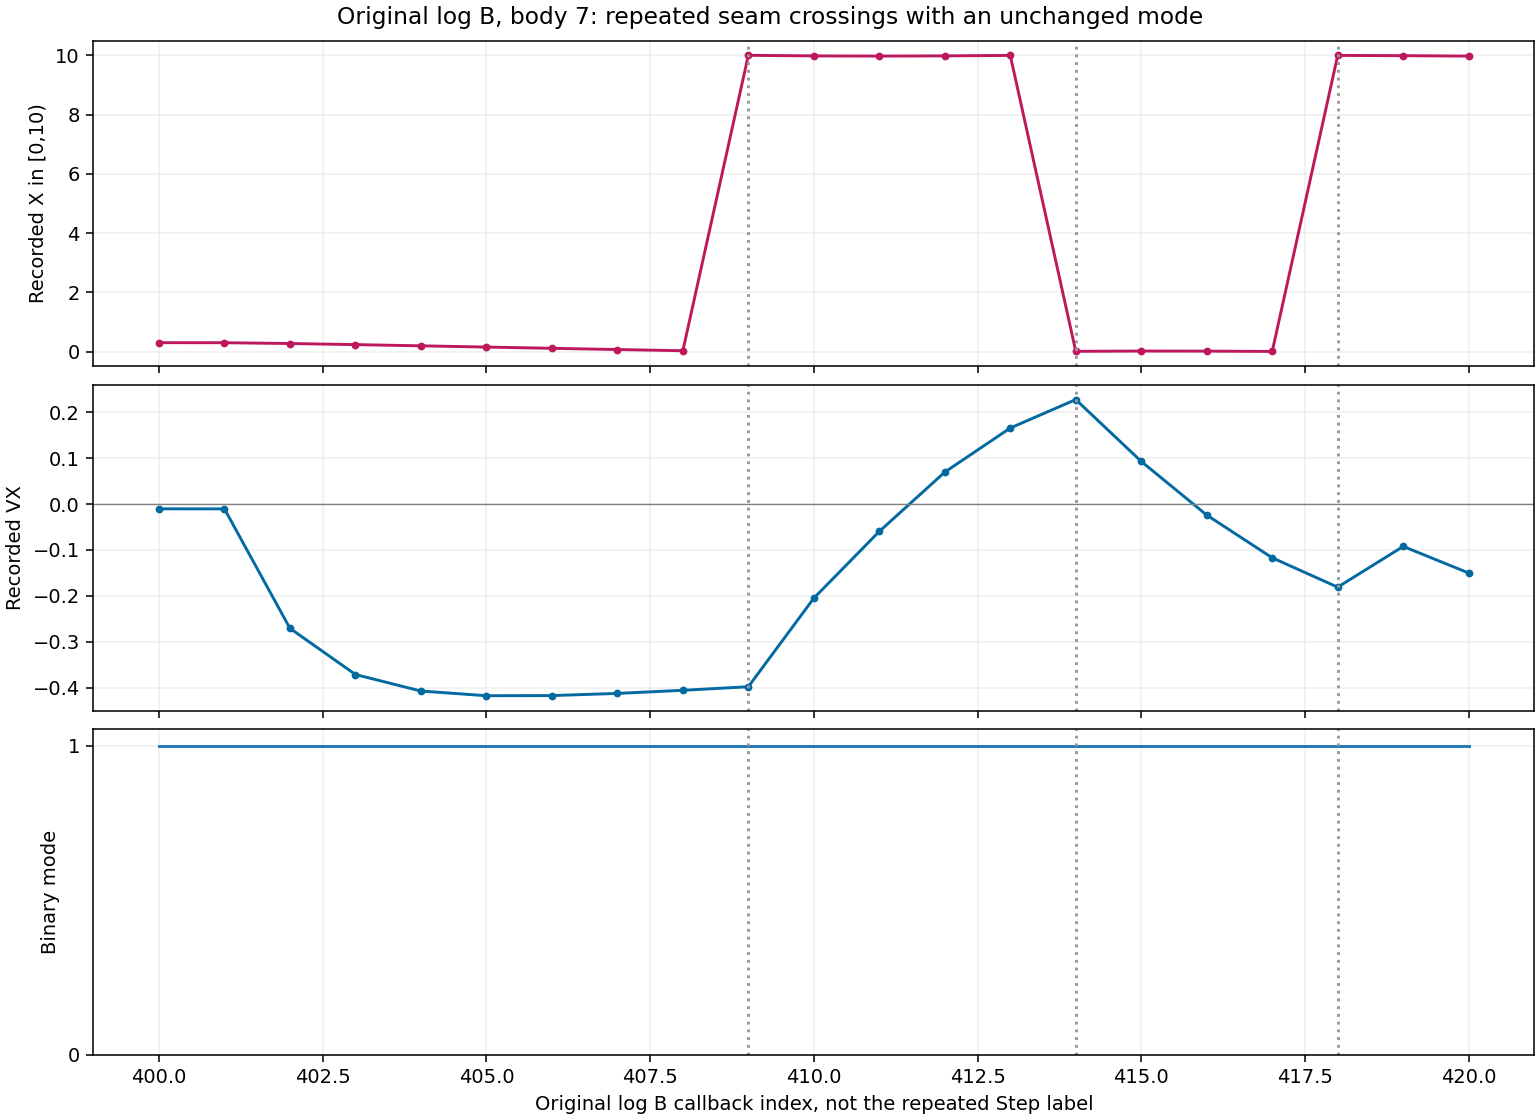
\includegraphics[width=\linewidth,height=0.70\textheight,keepaspectratio]{figures/F13_0.png}
\caption[Body 7 crosses the X seam with an unchanged mode]{DERIVED from ORIGINAL log B, body 7, q400--420. Panels show stored X, VX and mode. Seams at q409,414,418 correspond to CSV lines 3281,3321,3353; the mode remains 1 throughout this window. Coordinate jumps and actual VX sign changes are distinguishable. The later toggle at q431 is excluded. This finite episode is not a periodic-orbit proof. \cite{study03}}
\label{fig:F13}
\end{figure}
